\section{Application to Jigsaw Toxic Prediction Dataset}\label{sec:jigsaw}

In this section, we outline the methodology and findings related to the fine-tuning of the BERT model for toxic comment classification on the Jigsaw Toxic Prediction dataset. Building on the results from the Civil Comments Dataset, we narrowed the hyperparameter search space while considering dataset-specific characteristics, such as longer average comment lengths.

For this milestone, we focused exclusively on classifying the feature \texttt{toxic} to ensure comparability with the Civil Comments dataset. Multilabel classification tasks, which include other labels in the dataset, are planned to be addressed in Milestone 3.

\subsection{Feature selection and preprocessing}

Similar to the Civil Comments dataset, BERT's token, segment, and positional embeddings were used for the input representation. Tokenization was performed using the BertTokenizer and padding and truncation were applied to ensure uniform input sequence lengths. Given the longer average length of comments in the Jigsaw dataset, we retained the maximum sequence length of 512 tokens to preserve context and capture the semantic nuances of the data.

Preprocessing steps were evaluated but had minimal impact on model performance. Thus, raw input data without additional preprocessing was utilized, leveraging the robust tokenization and contextual embeddings provided by BERT.

\begin{figure}[ht] \centering 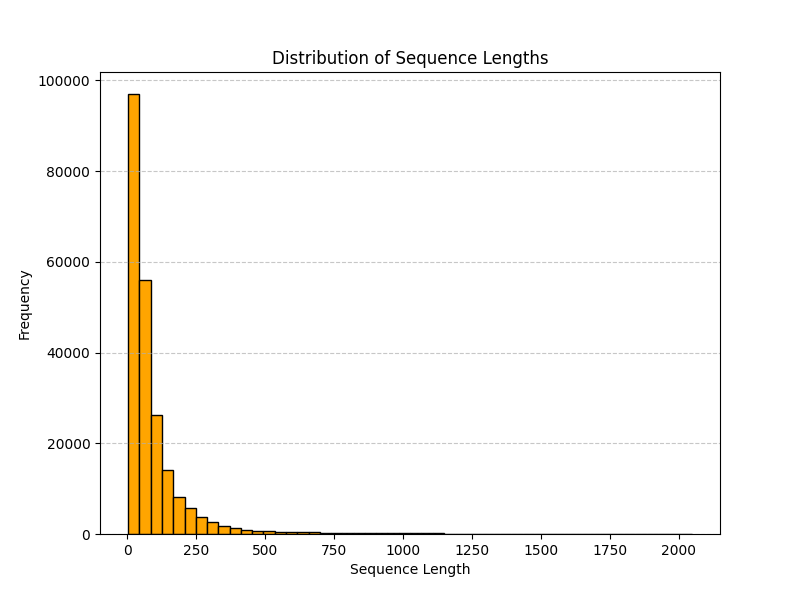
\includegraphics[width=0.8\textwidth]{./figures/jigsaw_seq_len.png} \caption{Distribution of comment lengths in Jigsaw Toxic Prediction dataset.} \label{fig:seq_len} \end{figure}

\subsection{Baseline and Fine-Tuning Methods}

We established a baseline using a logistic regression model with TF-IDF features, similar to the approach used for the Civil Comments dataset. This provided a point of comparison for evaluating the performance of the fine-tuned BERT model.

For fine-tuning, the BERT architecture was augmented with a classification head comprising a single fully connected linear layer. The logits from this layer were passed through a sigmoid activation function to yield probabilities for binary classification. The AdamW optimizer and BCEWithLogitsLoss were used for optimization and loss computation, respectively.

Due to the increased memory requirements caused by the longer sequence length (512 tokens), the batch size was reduced to 128. This adjustment was necessary to prevent memory overflow during training while maintaining efficient utilization of the hardware.

\subsection{Hyperparameter Search}

The hyperparameter search space was narrowed to focus on learning rate, number of epochs, and preprocessing, based on insights from the Civil Comments dataset. The chosen hyperparameter ranges were:

\begin{itemize} \item \textbf{Learning rate:} $[1 \times 10^{-6}, 1 \times 10^{-5}, 1 \times 10^{-4}, 1 \times 10^{-3}]$ \item \textbf{Number of epochs:} $[1, 5, 100]$ \item \textbf{Preprocessing:} $[\text{False}, \text{True}]$ \end{itemize}

\subsection{Findings}

\paragraph{Learning rate:} The optimal learning rate for this dataset was $1 \times 10^{-4}$. Extremely low or high values hindered convergence or caused instability during training.

\paragraph{Number of epochs:} Training for one epoch yielded comparable results to five epochs, consistent with findings from the Civil Comments dataset. This demonstrates the efficiency of fine-tuning pre-trained models for toxic comment classification tasks.

\paragraph{Preprocessing:} As with the Civil Comments dataset, preprocessing steps did not provide significant performance improvements. This confirms the robustness of BERT's tokenizer and pre-trained embeddings in handling raw input data.

\paragraph{Baseline Methods:} Baseline methods similar to those established for the Civil Comments dataset in Milestone 1 were implemented and evaluated. The best-performing baseline was selected for comparison. Additional results and details on baseline methods are available on GitHub. The results of the best baseline methods and the best BERT configuration are shown in the figure below.

\begin{figure}[ht] \centering 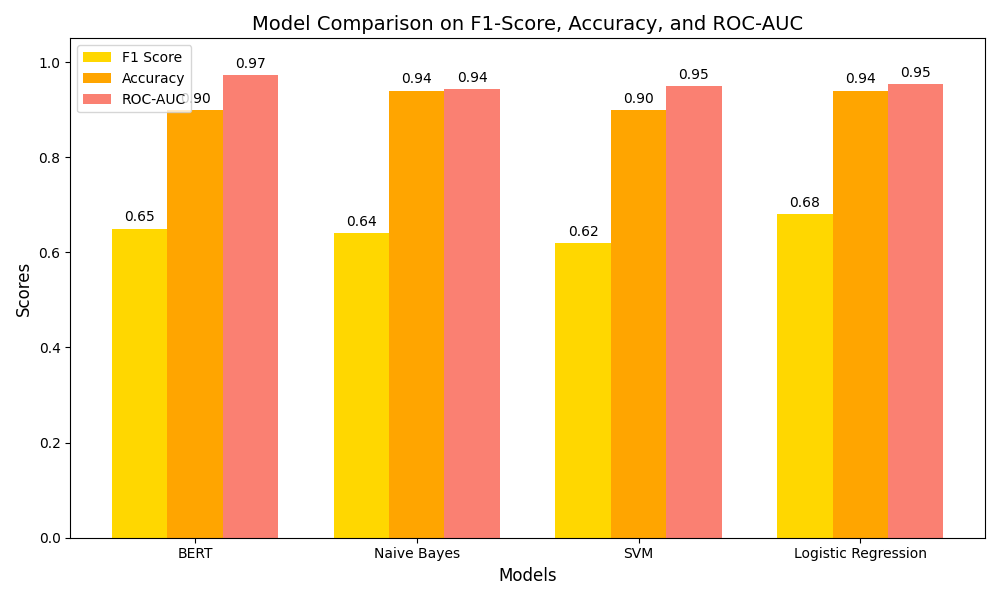
\includegraphics[width=0.7\textwidth]{./figures/jigsaw_baseline_bert_test.png} \caption{Models' performance on the Jigsaw test dataset.} \label{fig:performance_test_set_jigsaw} \end{figure}

\subsection{Comparison to Civil Comments Dataset}

The methodology for the Jigsaw dataset mirrored that of the Civil Comments dataset, with adjustments made to accommodate the longer average comment lengths. The narrower hyperparameter search space and use of a baseline enabled efficient experimentation while achieving high performance metrics. This iterative approach highlights the adaptability of the pipeline to datasets with differing characteristics.

\subsection{Conclusion of application on Jigsaw Dataset}

The same hyperparameter configuration that was found optimal for the Civil Comments dataset was also optimal for the Jigsaw Toxic Prediction dataset, except with a sequence length of 512 instead of 128 to accommodate the longer comment lengths. Furthermore, the batch size was set to 128 to handle memory limitations caused by the increased sequence length.

The BERT model outperformed the baseline methods on the Jigsaw dataset according to the ROC-AUC metric, which is the most important evaluation metric for this task. However, performance across other metrics was comparable between BERT and the baseline methods. This discrepancy is likely due to differences in the distribution of the test dataset compared to the training and validation datasets. On the validation datasets, BERT demonstrated a significantly stronger performance compared to the baseline methods. This setup ensures efficient fine-tuning while addressing the unique challenges posed by the dataset's characteristics.